% vim: set fenc=utf-8 ft=latex encoding=utf-8
% -*- mode: latex; coding: UTF-8; -*-

\newif\ifdraft
% \drafttrue

\ifdraft
        \documentclass[conference, draftclsnofoot, draft]{IEEEtran}
        \def\baselinestretch{1}
        \setlength{\marginparwidth}{2cm}
\else
        \documentclass[conference]{IEEEtran}
\fi

\usepackage[T1]{fontenc}
\usepackage[utf8]{inputenc}

\newcommand{\TheTitle}{Merge-tree: Visualizing the Integration of Commits into Linux}
\newcommand{\TheAuthors}{Evan Wilde, Daniel German}
\newcommand{\TheEmails}{etcwilde@uvic.ca, dmg@uvic.ca}
\newcommand{\TheSubject}{Digesting large amounts of commit data}
\newcommand{\TheKeywords}{Linux, git, data structures, tree data structures}

\synctex=1

\usepackage[hyphens]{url}
\urlstyle{same}

\ifdraft
        \usepackage[unicode=true,bookmarks=false,breaklinks=false,
                pdfborder={0 0 0},backref=none,colorlinks=true]{hyperref}

\else
        \usepackage[unicode=true,bookmarks=false,breaklinks=false,
                pdfborder={0 0 0},backref=none,colorlinks=false]{hyperref}
\fi

\usepackage[nospace]{cite}

% Table Support
\usepackage{dcolumn}
\usepackage{longtable}

\usepackage{balance}
\usepackage{placeins}
\usepackage{multirow}

% Extra support
\usepackage{xspace}
\usepackage{caption}
\usepackage[nospace]{cite}

\usepackage{amsmath}
\usepackage{algorithm}
\usepackage{algpseudocode}
\usepackage{tikz}
\usepackage{xcolor}
\usepackage{color}

% Fix any bad-hyphenations here
\hyphenation{contained}

% Tikz libraries
\usetikzlibrary{positioning}

% Chart Colors
\definecolor{chartblue}{HTML}{3366CC}
\definecolor{chartred}{HTML}{DC3912}
\definecolor{chartyellow}{HTML}{FF9900}
\definecolor{chartgreen}{HTML}{109618}
\definecolor{chartmagenta}{HTML}{990099}
\definecolor{chartpurple}{HTML}{3B3EAC}

% \ifdraft
%     \usepackage[colorinlistoftodos]{todonotes}
%     \newcommand{\evan}[1]{{\color{blue}\emph{Evan Says: #1}}\xspace}
%     \newcommand{\evantodo}[1]{{\color{blue}\emph{Evan Todo: #1}}\xspace}
%     \newcommand{\dmg}[1]{{\color{blue}\emph{dmg Says: #1}}\xspace}
%     \newcommand{\dmgtodo}[1]{{\color{blue}\emph{dmg Todo: #1}}\xspace}
% \else
%     \usepackage[disable]{todonotes}
%     \newcommand{\evan}[1]{}
%     \newcommand{\evantodo}[1]{}
%     \newcommand{\dmg}[1]{}
%     \newcommand{\dmgtodo}[1]{}
% \fi
    \usepackage[colorinlistoftodos]{todonotes}

\newcommand{\tool}{{\emph Linvis}\xspace}


    \newcommand{\evan}[1]{{\color{blue}\emph{Evan Says: #1}}\xspace}
    \newcommand{\evantodo}[1]{{\color{blue}\emph{Evan Todo: #1}}\xspace}
    \newcommand{\dmg}[1]{{\color{blue}\emph{dmg Says: #1}}\xspace}
    \newcommand{\dmgtodo}[1]{{\color{blue}\emph{dmg Todo: #1}}\xspace}


%%% Local Variables:
%%% mode: plain-tex
%%% TeX-master: t
%%% End:


\begin{document}

\title{\TheTitle}
\author{
        \IEEEauthorblockA{\TheAuthors}
        \IEEEauthorblockN{Department of Computer Science,
                University of Victoria, Canada.}
        \IEEEauthorblockA{Email: \TheEmails}
}
\maketitle
\begin{abstract}

With an average of more than 900 top-level merges into the Linux kernel per
release, many containing hundreds of commits and some containing thousands,
maintenance of older versions of the kernel becomes nearly impossible.
Various commercial products, such as the Android platform, run older
versions of the kernel. Due to security, performance, and changing hardware
needs, maintainers must understand what changes (commits) are added to the
current version of the kernel since the last time they inspected it in order
to make the necessary patches.

Current tools provide information about repositories through the directed
acyclic graph (DAG) of the repository, which is helpful for smaller
projects. However, with the scale and number of branches in the kernel the
DAG becomes overwhelming very quickly. Furthermore, the DAG contains every
ancestor of every commit, while maintainers are more interested in how and
when a commit arrives to the official Linux repository.

In this paper, we propose the merge-tree, a simplified transformation
of the DAG of the Linux git repository that shows the way in which commits
are merged into the master branch of Linux. Using the merge-tree, we
build \tool, a tool that is designed to allow users to explore how commits
are merged into the Linux kernel.

\end{abstract}

\begin{IEEEkeywords}
        \TheKeywords
\end{IEEEkeywords}


\section{Introduction}

Between 50k and 70k commits are added to the Linux kernel per version requiring
maintainers of older versions of the kernel to sift through thousands of
commits and merges with tools that are unable to filter and effectively visualize
projects at the scale of the kernel. Older versions of the kernel are used in
embedded systems and mobile phones; for security purposes, performance needs, and
changing hardware requirements, maintainers must be able to understand the changes
being made in the current version of the kernel in order to produce the necessary
patches for the older versions of the kernel. Tools like Gitk use a directed acyclic
graph (DAG) model of the repository, showing all commits and merges in chronological
order by when the commit was authored, not by when it arrived in the official Linux
repository.

\begin{figure*}
        \centering
        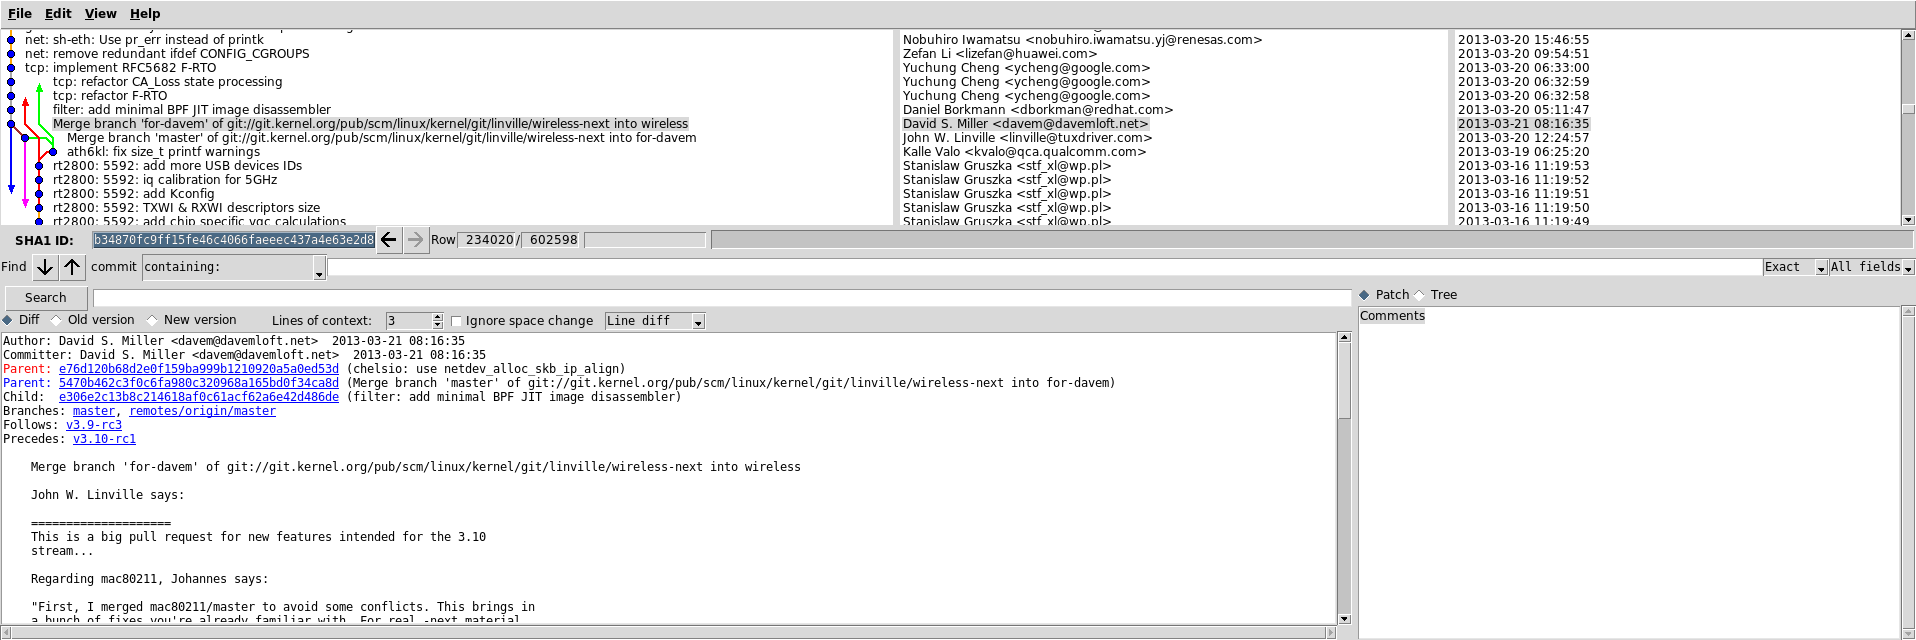
\includegraphics[width=0.97\textwidth]{figures/gitk.png}
        \caption{A view of the Gitk interface centered on merge
          b34870fc9ff15fe46c4066faeeec437a4e63e2d8 by Miller. Commits point toward
          their ancestors and there is no clear path from the commit to the merge
          with the master branch. Neither Gitk nor Git are capable of showing the
          commits in master.}
        \label{fig:gitk}
%\vspace{-4mm}
\end{figure*}


\begin{figure}
        \centering
        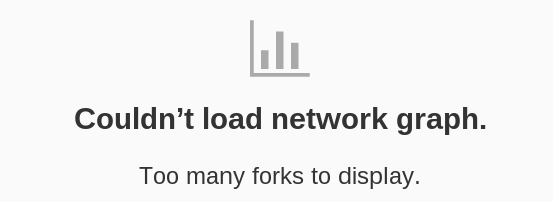
\includegraphics[width=0.45\textwidth]{figures/github_viewer.png}
        \caption{Github Failure Message showing the DAG of the Linux Project and its
                relationship to other forks.}
        \label{fig:gitfail}
%\vspace{-2mm}
\end{figure}


This representation works in smaller projects; it enables users to see when changes
are made, when these changes are merged, how each branch is interacting, and the
point where a branch forks from the master branch. In large modular projects, like
the Linux kernel, the DAG becomes a mess of merges and commits
(Figure~\ref{fig:gitk}) losing its visual meaning. In some cases, the Linux kernel
is simply too large for the system to generate a visualization; Github provides a
DAG view for many projects, but is unable to display the visualization for projects
at the scale of the Linux of the kernel (Figure~\ref{fig:gitfail}).  Between 60k and
70k new commits are created for the Linux project every year; according to our
previous work\cite{German2015}, a commit takes a median of 30 days from the time it
is authored until it arrives in the official repository. The snapshot of the kernel
tomorrow may be different than the snapshot from today, containing new commits
authored in the past; distinguishing these new commits from the commits in the
snapshot from today is not trivial.


One major challenge with visualizing the arrival of commits to a repository is that
Git does not store the date that a commit was merged into another branch, including
the master branch. To complicate the problem, the DAG only has references to the
ancestors of a commit (a model necessary for the operation of Git), but maintainers
would prefer knowing the path a commit followed to reach the master repository.
Tracing a path that any commit followed to the master repository would imply that
for any given merge, it would be possible to know which commits were merged. A user
could inspect the commits that arrived into the master branch within a given
time-frame by checking which commits were merged during that time-frame.

This paper makes two contributions; first, we describe a method of converting the
DAG of the Linux repository into a tree, or \emph{merge-tree} of the repository,
that represents the path used by a commit to reach the master branch; second, we
present a method to inspect and visualize the history of merges in the Linux project
using the merge-tree model.

These methods and visualizations are implemented in a web-based tool called
\tool\footnote{\tool is currently available at \url{http://li.turingmachine.org}}.
Our visualizations and tool provide information about the location of any given
commit or merge in its respective merge-tree, the files edited, the modules edited,
and the commit message. \tool allows users to apply various filters, including the
release version, along with a keyword or phrase from the log preview, the name of
the author, or the commit ID. The user can request all merges made by Linus that
contain a commit or inner merge that matches the search query, or just the commits
and merges that match the query.

\section{Merge-Tree model}
\label{sec:mergetree}

Git uses a directed acyclic graph (DAG) as its main data model. In this model, a
commit has one or more ordered parents (ancestors), except the root commits of a
repository which do not have ancestors--Linux's git repository has two such commits.
Commits are divided into merge commits, merging two or more branches, and non-merge
commits. Non-merge commits have only one parent, while merge commits have two or
more. The order of the parents matter: the first parent is the branch in which the
merge is being done, while the rest indicate the branches being merged (Git allows
merging multiple branches simultaneously). The second parent is the first branch
merged, the third parent is the second branched merged, etc.

Once a commit is created, it is never changed. Git allows operations to alter
commits or reorder them, but it changes the commit ID in the process, effectively
replacing it with a new commit. This makes commits unable to record the traversal of merges
from the commit to the merge into the master branch.

A short example: assume the commits represented in Figure~\ref{fig:repoEvents} show
the sequence of events in a repository. In this case, commits are performed in
various repositories and branches. The DAG representation of the commits is shown in
Figure~\ref{fig:repoDAG}. Notice that the DAG loses information about the master
branch and the repository that the master branch is part of. The merge-tree view of
this DAG is visible in Figure~\ref{fig:repoTree}. Note that the direction of the
edges of the DAG have been inverted, instead of pointing from the child to the
ancestors, it points from the ancestor to its successors, forming a path to the
master branch. Also note that the DAG has been simplified, showing only a single
edge on the path to master for any commit.

\begin{figure}[htbp]
  \centering
  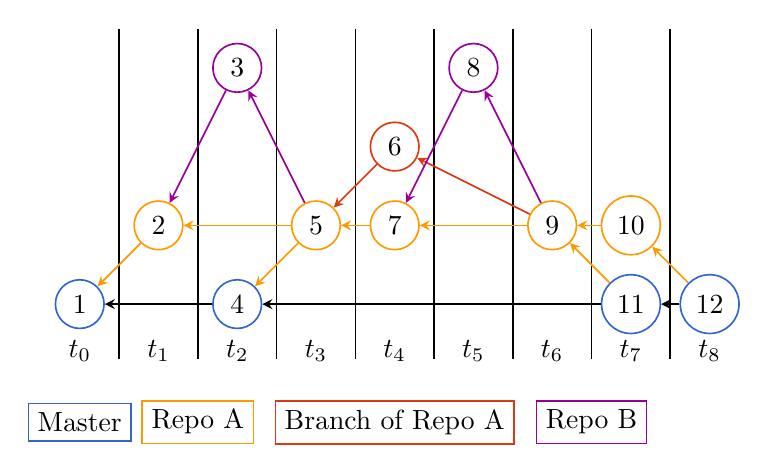
\begin{tikzpicture}[auto, on grid, semithick, state/.style={circle, text=black}]
    \foreach \x in {0, 1, 2, 3, 4, 5, 6, 7}
    \draw[shift={(\x + 0.5, -0.5)}, color=black] (0cm, 4cm) -- (0pt, -0.2cm);

    \node[state, draw=chartblue] (1) {1};
    \node[state, draw=chartyellow, above right= of 1] (2) {2};
    \node[state, draw=chartmagenta, above right= 2cm and 1cm of 2] (3) {3};
    \node[state, draw=chartblue, right= 2cm of 1] (4) {4};
    \node[state, draw=chartyellow, above right=of 4] (5) {5};
    \node[state, draw=chartred, above right=of 5] (6) {6};
    \node[state, draw=chartyellow, right=of 5] (7) {7};
    \node[state, draw=chartmagenta, above right= 2cm and 1cm of 7](8) {8};
    \node[state, draw=chartyellow, right= 2cm of 7] (9) {9};
    \node[state, draw=chartyellow, right=of 9] (10) {10};
    \node[state, draw=chartblue, below right=of 9] (11) {11};
    \node[state, draw=chartblue, below right=of 10] (12) {12};

    \draw (12) edge[-stealth] (11) edge[chartyellow, -stealth] (10);
    \draw (11) edge[-stealth] (4) edge[chartyellow, -stealth] (9);
    \draw (10) edge[chartyellow, -stealth] (9);
    \draw (9) edge[chartmagenta, -stealth] (8) edge[chartred, -stealth] (6)
              edge[chartyellow, -stealth] (7);
    \draw (8) edge[chartmagenta, -stealth] (7);
    \draw (7) edge[chartyellow, -stealth] (5);
    \draw (6) edge[chartred, -stealth] (5);
    \draw (5) edge[chartmagenta, -stealth] (3) edge[chartyellow,-stealth] (2)
              edge[chartyellow, -stealth] (4);
    \draw (4) edge[-stealth] (1);
    \draw (3) edge[chartmagenta, -stealth] (2);
    \draw (2) edge[chartyellow, -stealth] (1);

    \node [draw=chartblue, below = 1.5cm of 1] (l1) {Master};
    \node [draw=chartyellow, right = 1.5cm of l1] (l2) {Repo A};
    \node [draw=chartred, right = 2.5cm of l2] (l3) {Branch of Repo A};
    \node [draw=chartmagenta, right= 2.5cm of l3] (l4) {Repo B};

        \foreach \x in {0, 1, 2, 3, 4, 5, 6, 7, 8}
    \node[shift={(\x, -0.6)}, color=black] {$t_\x$};
  \end{tikzpicture}
  \caption{Example of a sequence of events performed in different
    repositories. The horizontal axis represents time. Each horizontal
    section represents a different branch and/or repository. Each commit
    points to its ancestor.}
  \label{fig:repoEvents}
%\vspace{-3mm}
\end{figure}

\begin{figure}[htbp]
  \centering
  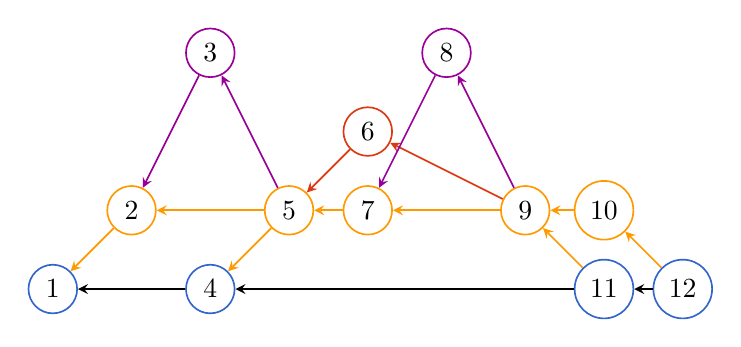
\begin{tikzpicture}[auto, on grid, semithick, state/.style={circle, text=black}]
    \node[state, draw=chartblue] (1) {1};
    \node[state, draw=chartyellow, above right= of 1] (2) {2};
    \node[state, draw=chartmagenta, above right= 2cm and 1cm of 2] (3) {3};
    \node[state, draw=chartblue, right= 2cm of 1] (4) {4};
    \node[state, draw=chartyellow, above right=of 4] (5) {5};
    \node[state, draw=chartred, above right=of 5] (6) {6};
    \node[state, draw=chartyellow, right=of 5] (7) {7};
    \node[state, draw=chartmagenta, above right= 2cm and 1cm of 7](8) {8};
    \node[state, draw=chartyellow, right= 2cm of 7] (9) {9};
    \node[state, draw=chartyellow, right=of 9] (10) {10};
    \node[state, draw=chartblue, below right=of 9] (11) {11};
    \node[state, draw=chartblue, below right=of 10] (12) {12};

    \draw (12) edge[-stealth] (11) edge[chartyellow, -stealth] (10);
    \draw (11) edge[-stealth] (4) edge[chartyellow, -stealth] (9);
    \draw (10) edge[chartyellow, -stealth] (9);
    \draw (9) edge[chartmagenta, -stealth] (8) edge[chartred, -stealth] (6)
              edge[chartyellow, -stealth] (7);
    \draw (8) edge[chartmagenta, -stealth] (7);
    \draw (7) edge[chartyellow, -stealth] (5);
    \draw (6) edge[chartred, -stealth] (5);
    \draw (5) edge[chartmagenta, -stealth] (3) edge[chartyellow,-stealth] (2)
              edge[chartyellow, -stealth] (4);
    \draw (4) edge[-stealth] (1);
    \draw (3) edge[chartmagenta, -stealth] (2);
    \draw (2) edge[chartyellow, -stealth] (1);
  \end{tikzpicture}
  \caption{DAG representation of the commits represented in
    Figure~\ref{fig:repoEvents}. The DAG loses information about which
    repository the commit is performed in and through which merges it
    has passed on its way to the master branch. The DAG does not even
    distinguish the master branch from other branches.}
  \label{fig:repoDAG}
%\vspace{-3mm}
\end{figure}

\begin{figure}[htbp]
  \centering
  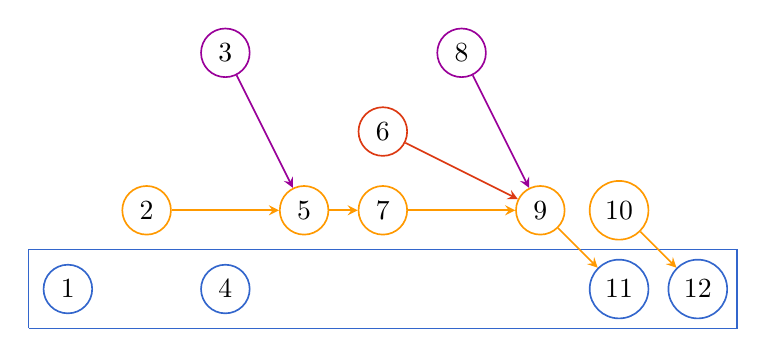
\begin{tikzpicture}[auto, on grid, semithick, state/.style={circle, text=black}]

    \draw[chartblue]
      (-0.5, -0.5) -- (8.5, -0.5) -- (8.5, 0.5) -- (-0.5, 0.5) -- (-0.5, -0.5);

    \node[state, draw=chartblue] (1) {1};
    \node[state, draw=chartyellow, above right= of 1] (2) {2};
    \node[state, draw=chartmagenta, above right= 2cm and 1cm of 2] (3) {3};
    \node[state, draw=chartblue, right= 2cm of 1] (4) {4};
    \node[state, draw=chartyellow, above right=of 4] (5) {5};
    \node[state, draw=chartred, above right=of 5] (6) {6};
    \node[state, draw=chartyellow, right=of 5] (7) {7};
    \node[state, draw=chartmagenta, above right= 2cm and 1cm of 7](8) {8};
    \node[state, draw=chartyellow, right= 2cm of 7] (9) {9};
    \node[state, draw=chartyellow, right=of 9] (10) {10};
    \node[state, draw=chartblue, below right=of 9] (11) {11};
    \node[state, draw=chartblue, below right=of 10] (12) {12};

    \draw (2) edge[chartyellow, -stealth] (5)
          (3) edge[chartmagenta, -stealth](5)
          (5) edge[chartyellow, -stealth] (7)
          (7) edge[chartyellow, -stealth] (9)
          (6) edge[chartred, -stealth] (9)
          (8) edge[chartmagenta, -stealth] (9)
          (9) edge[chartyellow, -stealth] (11)
          (10) edge[chartyellow, -stealth] (12);


  \end{tikzpicture}
  \caption{Merge-tree view of the commits  represented in
    Figure~\ref{fig:repoEvents} showing the path they followed to reach
    the master branch. In this model the successors of each commit
    represents the path followed by that commit to reach the master
    branch.}
  \label{fig:repoTree}
\vspace{-3mm}
\end{figure}

\subsection{Computing the merge-tree of the DAG of Linux}

Computing the merge-tree from a DAG for any repository may not be possible; however,
certain features of the development process of Linux make it feasible to compute the
merge-tree for the Linux repository. First, the master branch of Linux is maintained
by Linus Torvalds, and only Linus has write access to it. We have verified this
assertion in previous research~\cite{German2015}. We have developed a heuristic that
is presented in Algorithm~\ref{fig:alg}. In short, the algorithm first identifies
the commits made directly to the master branch; whereafter it recursively determines
the shortest path (in terms of time), using the DAG, from each commit to the master
branch using the inverted DAG.

\begin{algorithm}
        \caption{Computing the merge-tree of Linux Git's DAG}\label{fig:alg}
        \begin{algorithmic}
                \Function{ComputeMergeTree}{DAG}: tree
                \State {\# Compute the tree from the DAG of Linux repository.}
                \State {\# Returns $Tree$, a graph containing every commit }
                \State {\# in DAG with the path it followed to master.}

                \State $head \gets \textit{Head of master of git repository}$
                \State $master \gets \textit{traverse DAG from head using }$
                \State \quad\quad\quad\quad $\textit{first ancestor until reaching root}$
                \State $nodes(Tree) \gets nodes(DAG)$
                \State \Function{distance2Master}{cid} : seconds
                \State {\# Helper function}
                \State {\# Recursively compute shortest distance to master}
                \State {\# setting cid's successor (next) in its way to master.}
                \State {\# This function should be memoized. Otherwise it}
                \State {\# would run in exponential time.}
                \If {\textit{cid in master}}
                \State \Return 0
                \EndIf
                \State    $d \gets 	\infty$
                \State {\# Traverse the inverted DAG}
                \For{$c \in children(cid, DAG)$}
                \If {$c \in master$}
                \State $d_1 \gets commitTime(c)-commitTime(cid)$
                \Else
                \State {$d_1 \gets distance2Master(c)$}
                \EndIf
                \If {$d_1 < d $}
                \State $next \gets c$
                \State  $d \gets d_1$
                \EndIf
                \EndFor
                \State {\# $c$ is the commit that follows $cid$}
                \State {\# in its way to master}
                \State add edge $(cid, next)$ to $Tree$
                \State \Return $d$
                \EndFunction

                \State {\# Compute the distance for each commit}
                \State {\# discarding result}
                \For{$c \in nodes(DAG)$}
                \State $distance2Master(c)$
                \EndFor
                \State \Return $Tree$
                \EndFunction
        \end{algorithmic}
\end{algorithm}

\subsection{Evaluation}

Merges that do not have conflicts provide information to verify this heuristic. If a
merge does not contain a conflict, it records a summary of the commits that it
merges. See Figure~\ref{fig:sampleMerge} for an example. This summary contains a
list of the first 20 non-merge commits in the merge, including their one-line log
description, the full logs of the merge commits that merge this subset, and the
total number of non-merge commits in the merge.

\begin{figure}[htbp]
        \centering
        {\fontsize{7}{9}
        \begin{verbatim}
Merge: 8cbd84f fd8aa2c
Author: Linus Torvalds <torvalds@linux-foundation.org>
Date:   Tue Aug 10 15:38:19 2010 -0700

Merge branch 'for-linus' of git://neil.brown.name/md

* 'for-linus' of git://neil.brown.name/md: (24 commits)
md: clean up do_md_stop
[... edited for the sake of space]
md: split out md_rdev_init
md: be more careful setting MD_CHANGE_CLEAN
md/raid5: ensure we create a unique name for kmem_cache...
...
        \end{verbatim}}\vspace{-5mm}
        \caption{Example of how merges record a subset of commits being merged. The
                commit only shows the first 20 one-line summaries messages for the 24
                non-merge commits it merged. The ending ``...'' is part of the log
                and represents that other commits were merged.}
        \label{fig:sampleMerge}
\end{figure}



We used this information to evaluate the accuracy of the merge-tree model extracted from the DAG. The method we followed
started with the extraction of the commit history up to July 20, 2016. We computed the merge tree of every commit until
then. Since Linus Torvalds mostly does merging directly into master, we assumed that every merge by him is the root of a
merge-tree. As described above, the log of a merge-commit usually contains the number of commits in the merge the first 20
summaries of commits being merged. We extracted merges by Linus Torvalds using the command \mycode{log --merges --author='Torvalds} and compared
the number of commits according to the log with the number of commits in the  merge-tree rooted in this commit. We
also used the summaries of the commits found in the merge (not necessarily all---see above) to make sure those
commits were in their corresponding merge tree. For example, for the merge in
Figure~\ref{fig:sampleMerge} we would expect
that the merge tree rooted at \mycode{8cbd84f} contains 24 commits, and the one-line summaries corresponds to commits in
that merge-tree. We also inspected those with differences to make sure they were true errors.
The results can be summarized as follows:

\begin{itemize}
\item Five merges were false-errors because their logs did not contain accurate information (were probably edited by
  hand). For example in \mycode{42a579a0f...} one commit summary was missing (the line was empty), in \mycode
  {c55d267} the summaries were reordered.
\item The heuristic correctly identified that 79 of Linus merges (between Jun 7, 2014 and Jun 2, 2014) were made to a
  branch (not master). This branch was merged at (\mycode{3f17ea6d..} which contained 6809 commits.
\item The heuristic worked perfectly until Sept 4, 2007, the earliest date that it could be verified.
  Before this date, and until Dec 12, 2006, merges did not include a summary of the commits they included, hence making it
  impossible to verify; during this period, however, we correctly identified the merges by Linus into master.
\item Before Dec. 12, 2006 (1542 merges) our heuristic breaks due to the
presence of a \textit{foxtrot} commit (\mycode{c436688...}), which confounded the true master branch of a
repository (see \url{http://bit-booster.blogspot.ca/2016/02/no-foxtrots-allowed.html} for a description of the issue).
\end{itemize}

In summary, of the merges after Sept 4, 2007, in 100\% of them (16,860) our heuristic was correct. It failed in 1,542
commits before Dec. 12, 2006 and in 836 it appears to be correct (Dec 7, 2006 to Sept 4, 2007).

\section{Visualizing the merge-tree of Linux}

The goal of \tool is to simplify the navigation of the kernel commit information,
specifically focusing on merges. This is done by leveraging the merge-tree to
inspect how commits are merged on the path to the master repository.

\subsection{Use cases}

We designed \tool with two use-cases in mind, though a user may switch between the
cases as they work.

\noindent \textbf{Use-case 1: top-to-bottom approach}\label{sec:usecase1}\\ These
are users that are maintaining a section of the kernel and would like to pick a
merge (including all the commits that it merges) and merge it directly into their
current repository. This is useful for reducing the amount of re-implementation
work. For these users, it is important to have the ability to aggregate metadata
about files and modules being effected by the merge. Also, it is important for these
users to be able to navigate from the root of the merge-tree toward the leaves.

\noindent \textbf{Use-case 2: bottom-to-top approach}\label{sec:usecase2}\\
These are users that start with a known merge or commit and would like to see what
other changes are being made in commits that are in the same merge, including
knowing the merge-tree they belong to. This is useful to see what other commits are
related to the current commit and how they get collated into merges that eventually
end in the master branch. This is primarily for maintainers that need to perform
some specific cherry picking of commits. We must provide these users a mechanism for
navigating from a single commit toward the master branch, allowing them to see other
commits that might be related to their original commit.

\subsection{Data Model}

In our visualizations, we leverage the merge-tree model described in
Section~\ref{sec:mergetree}. In this model each commit is either already in the
master branch, or is part of a tree which is rooted in the merge that merged it into
the master branch.  Each commit, whether a merge or non-merge, has only one
successor; the root of each tree has none as it was made by Linus Torvalds directly
into the master branch. Non-merge commits contain the metadata for the changes made.
This metadata includes the files changed, the lines added and removed from each
file, the author, the date the commit was merged into the merge that led to being
merged into the kernel, the date the commit was authored, the patch, and the commit
log. Merges contain less metadata, only storing the author of the merge, the log,
the commit date, and the author date, and potentially, changes necessary to address
conflicts during the merge. The details of the model are outlined in
\cite{German2015}.

\section{Design and Implementation}

To navigate and inspect the merge-tree view of the kernel we created a web-based
tool called \tool. Creating a web-based tool enables users to use the system without
having to install additional software or store a large database, making it more
accessible, more easily maintainable, and platform independent. \tool uses the
following mechanisms to reach our goals of better navigation and better explanation
of the selected changes.

\begin{itemize}
        \item Filter by searching
        \item View files edited
        \item View modules
        \item Tree viewer
\end{itemize}

\subsection{Searching}

\begin{figure}
        \centering
        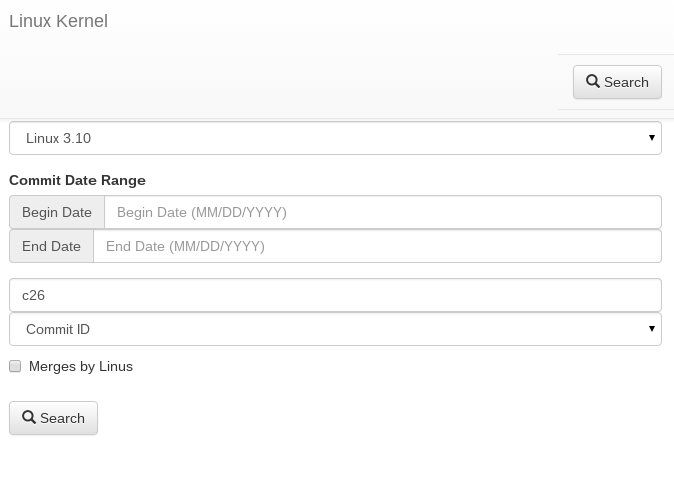
\includegraphics[width=0.47\textwidth]{figures/search.png}
        \caption{Search View allows filtering commits that were merged in a given
                period, filtering by author, keyword, or commit ID.}
        \label{fig:search}
\end{figure}

Searching (depicted in Figure \ref{fig:search}) allows a user to filter commits and
merges that are irrelevant. The search mechanism breaks down the results by release
version. A user can further narrow down the search by specifying a range of dates in
which such commits were merged by Linus into the master branch---not when the commits
were created (author date and/or commit date). This distinction is important. We have observed commits that have
taken years to arrive into the master repository after they were originally
created.

A user may then provide a search text, filtering by the author name, the commit ID,
or keyword from the log. Any part of the author name may show up in the results,
including searching by email address.

If the user is searching by commit ID, the ID can be specified by using any of its unique prefixes. For example, the commit
\mycode{3f17ea6dea8ba5668873afa54628a91aaa3fb1c0} is returned when the user searches for a
commit ID of \mycode{3f17e} in the 3.16 Linux kernel.

\begin{figure}
        \centering
        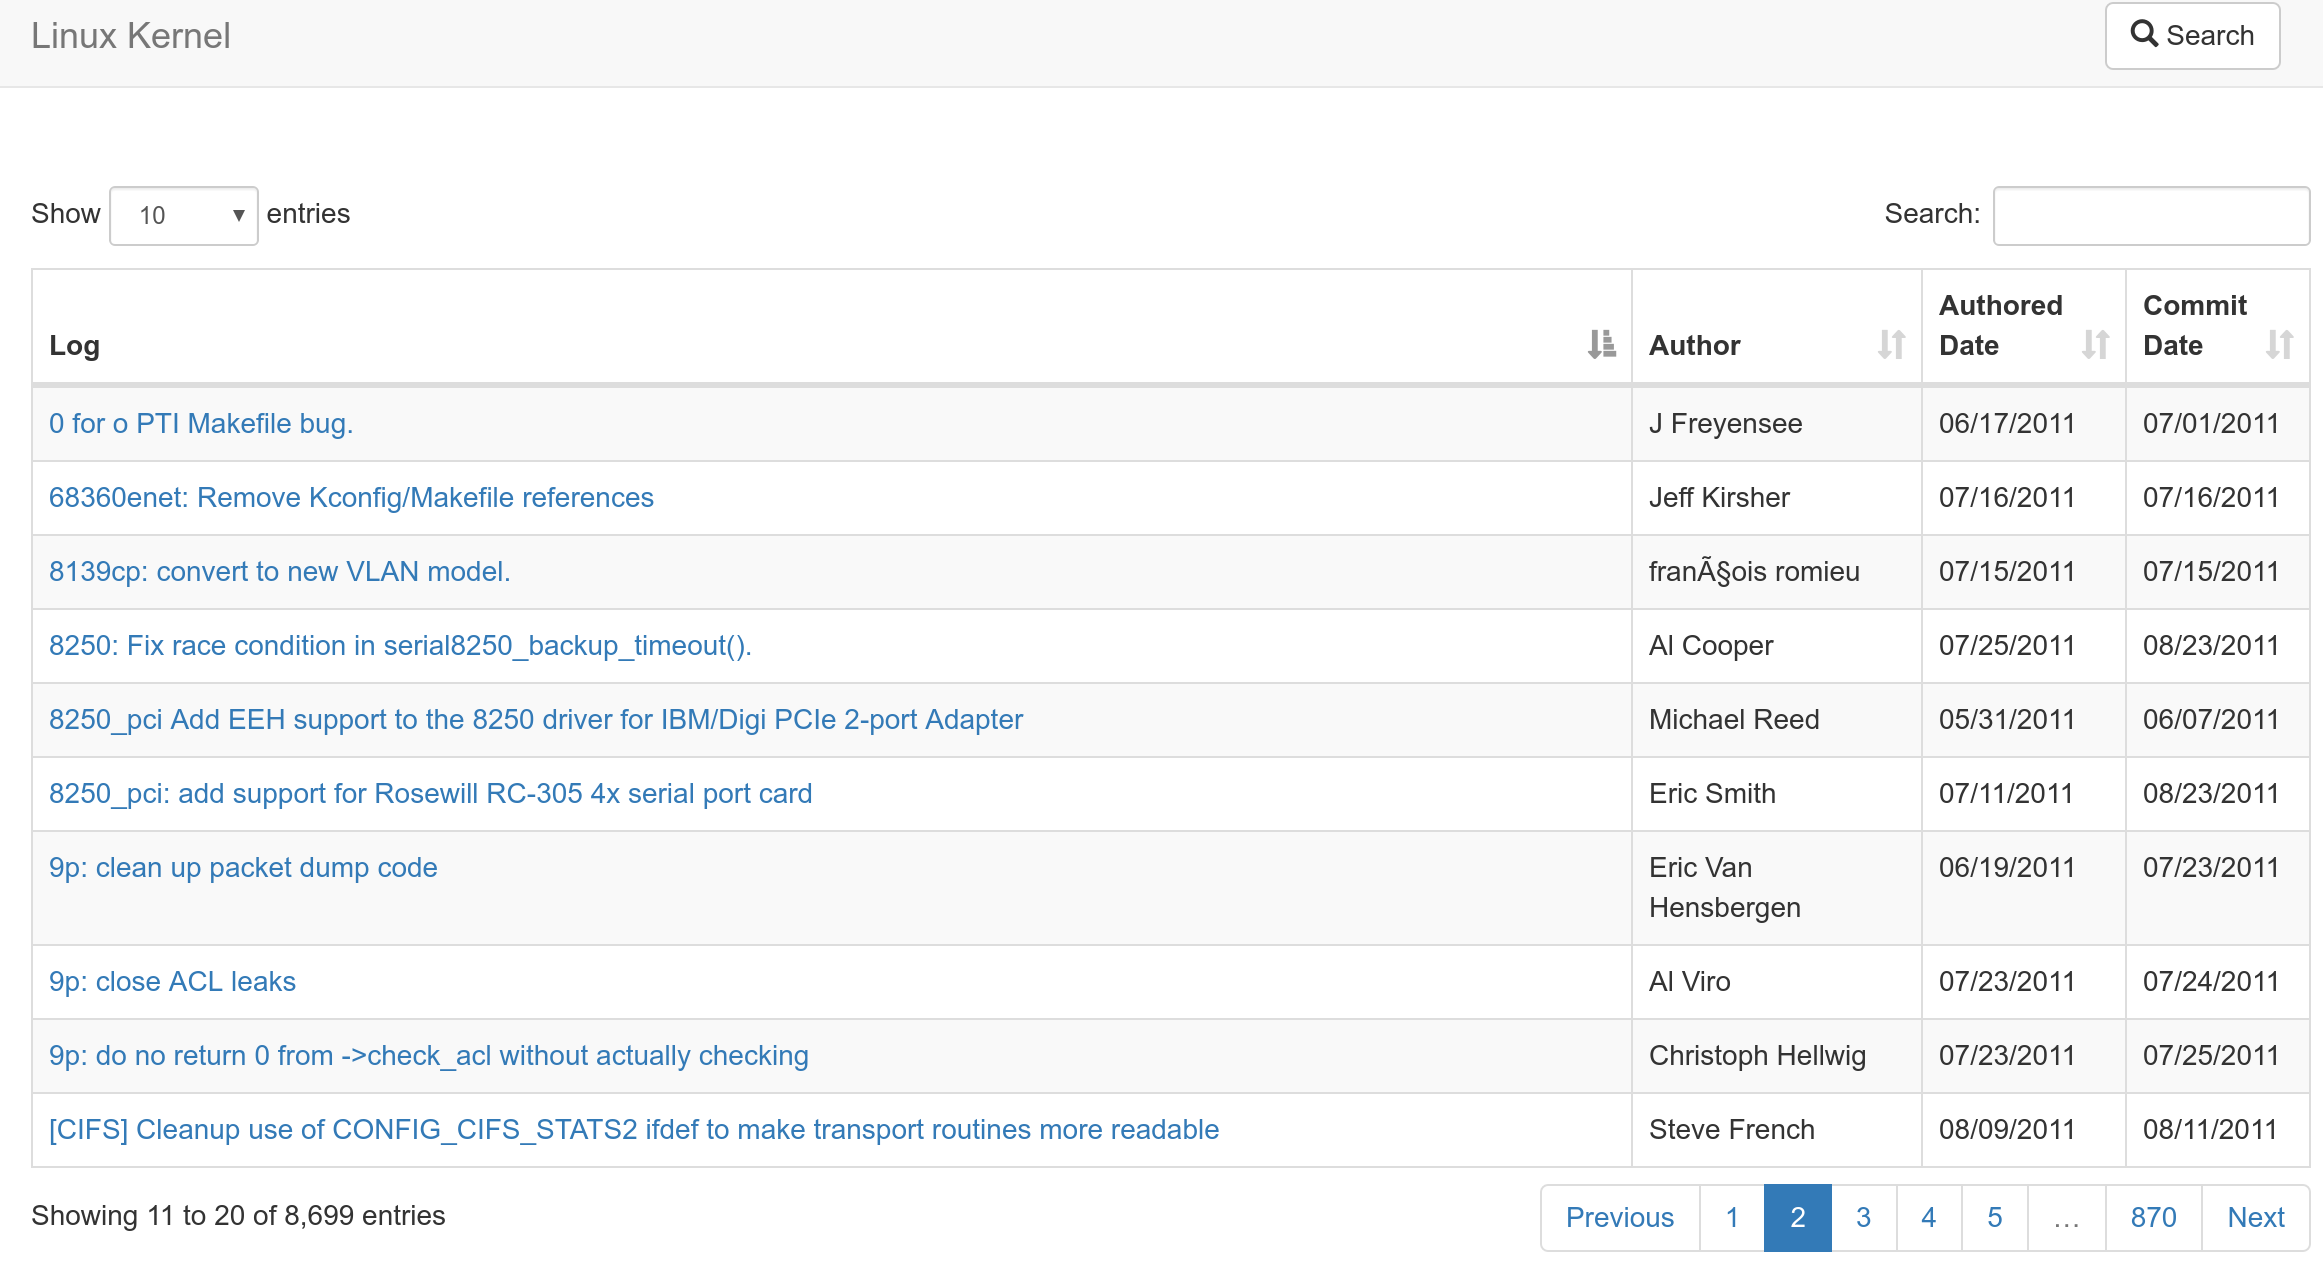
\includegraphics[width=0.47\textwidth]{figures/search_results_2.png}
        \caption{Search Results. Each table entry is a commit merged in the desired
                merged window.}
        \label{fig:results}
\end{figure}

In the search results (seen in Figure~\ref{fig:results}), the user is presented with the one-line log message preview,
the author's name and email, the date the commit was authored, and the date the commit was last committed.

\begin{figure}
        \centering
        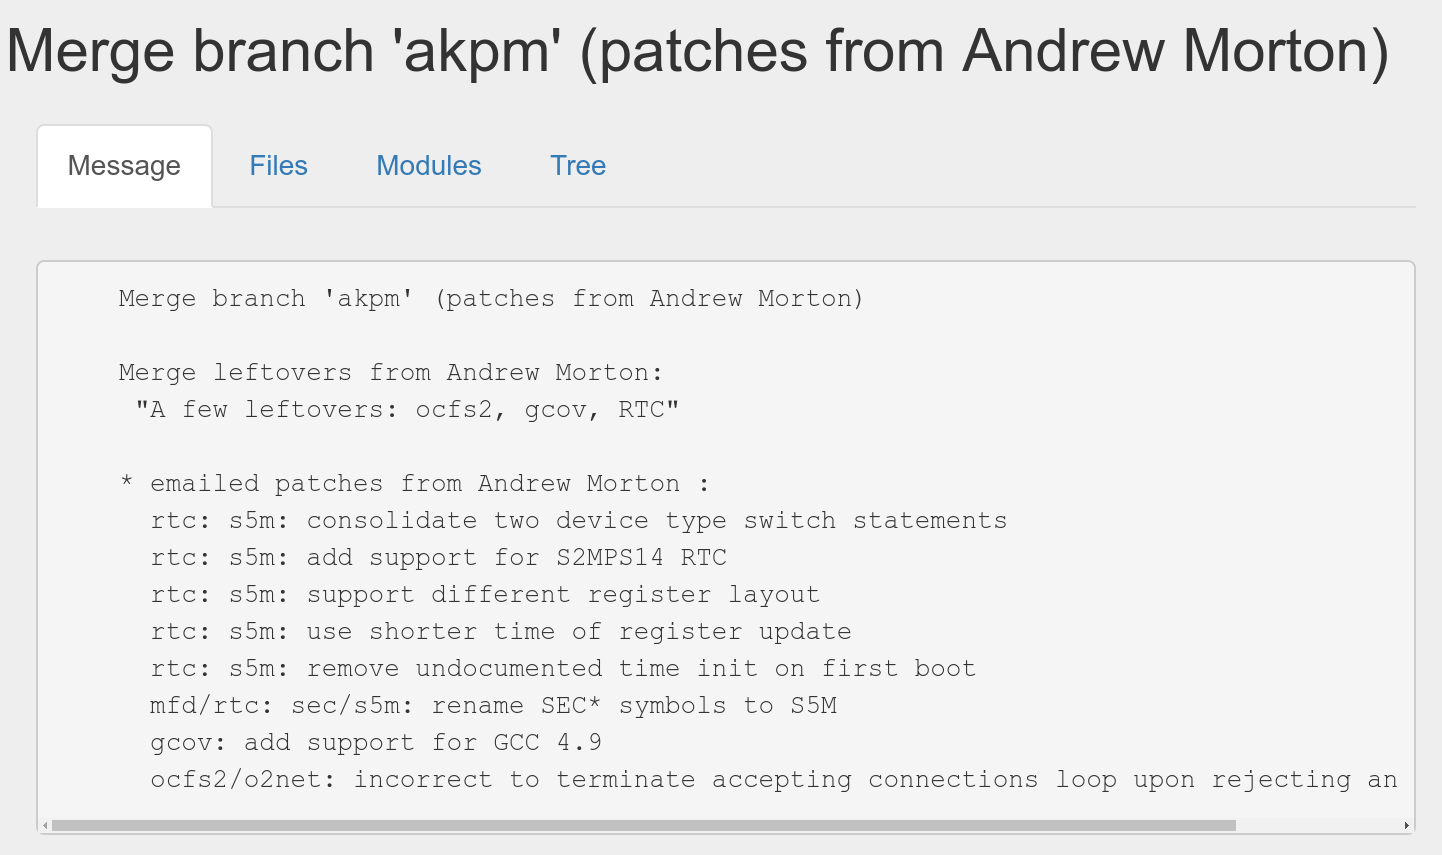
\includegraphics[width=0.47\textwidth]{figures/log_view.png}
        \caption{Panel showing the Commit Message of a commit.}
        \label{fig:message}
\end{figure}

Once a user selects a commit or merge to investigate, they are presented with a
tabbed pane allowing them to view the full commit log, the files edited, the modules
involved, and the merge-tree view.

The first tab displays the full commit log (Figure~\ref{fig:message}). From this, a
user is able to see what they would see had they searched for the commit using Git
log. This doesn't provide additional information to the other tools, but helps to
complete the functionality of \tool. The commit log provides a user with the
information about the content of the commit and who has signed-off on the commit to
ensure that it is of good quality. The message for merges may contain a summary of
the commits being merged.  The information within these messages is highly variable,
and is completely dependent on the author's style. As the user moves toward the
root-level merge, the quality of these messages generally improves.

\begin{figure}
        \centering
        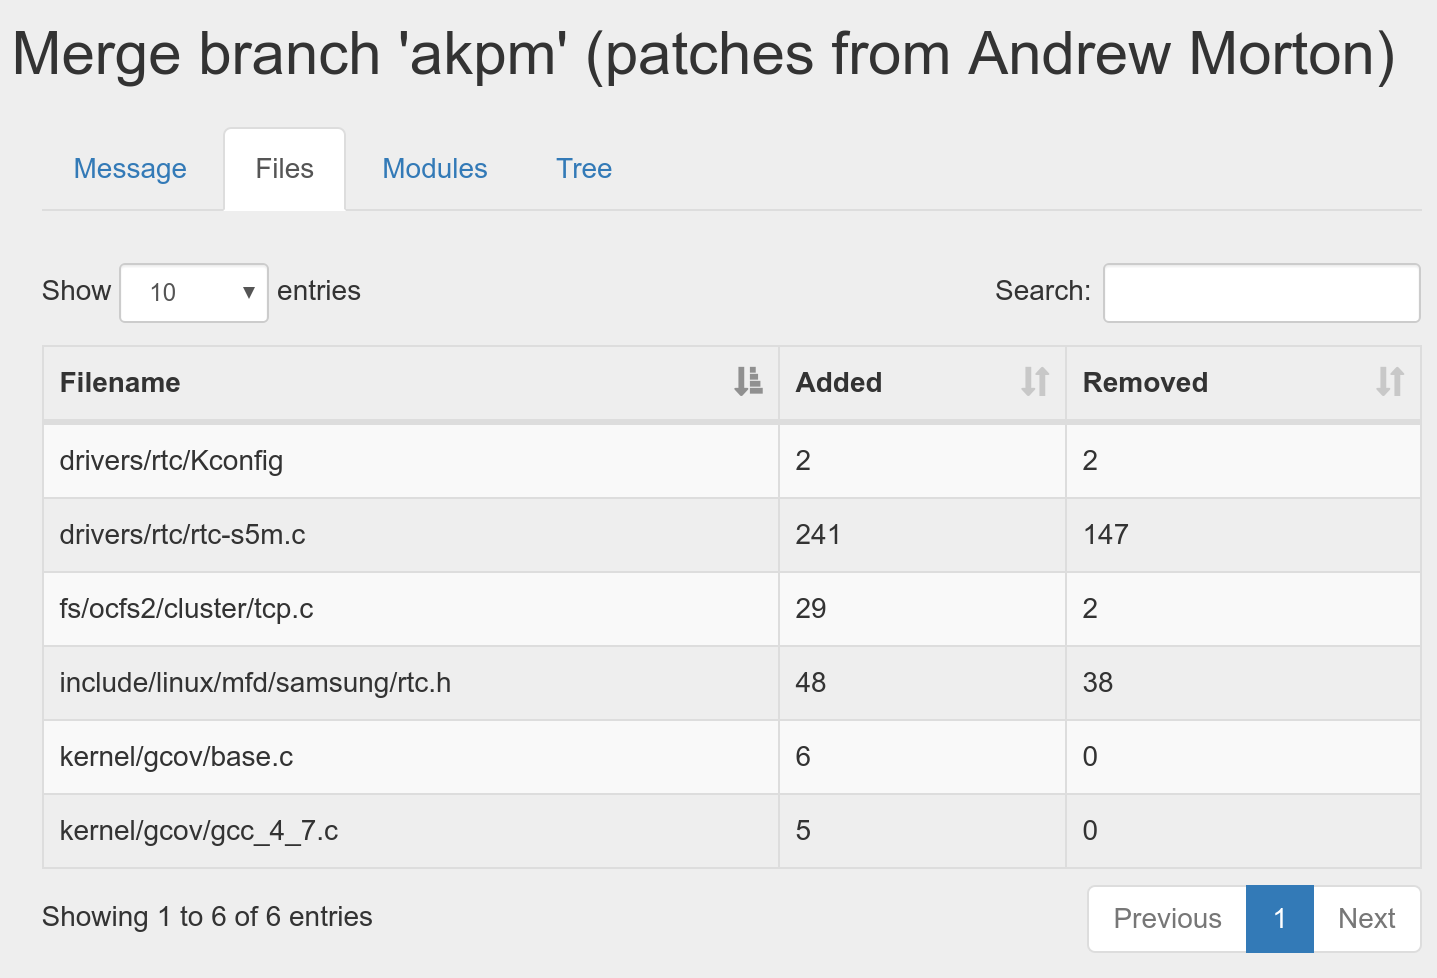
\includegraphics[width=0.47\textwidth]{figures/files_view_2.png}
        \caption{Panel showing the files modified by all the commits that are part
                of this merge.}
        \label{fig:files}
\end{figure}

The second tab is the files tab (Figure~\ref{fig:files}). This tab provides
information on what files have been edited, how many lines were added, and how many
lines were removed in a given commit. For non-merges, this functionality is similar
to the other tools available. Our tree-based design model allows us to extend this
functionality to merges by aggregating information about all the commits that are
children of the merge in the merge-tree, which other tools are unable to show. To
find the number of lines added to a file in a merge, we take the sum of the lines
added to that file in each of the children of that merge. We do the same for
calculating the number of lines removed.


% This could be extended to use the patch information to determine when a line has been
% replaced rather than incrementing the lines added and removed.

\begin{figure}
        \centering
        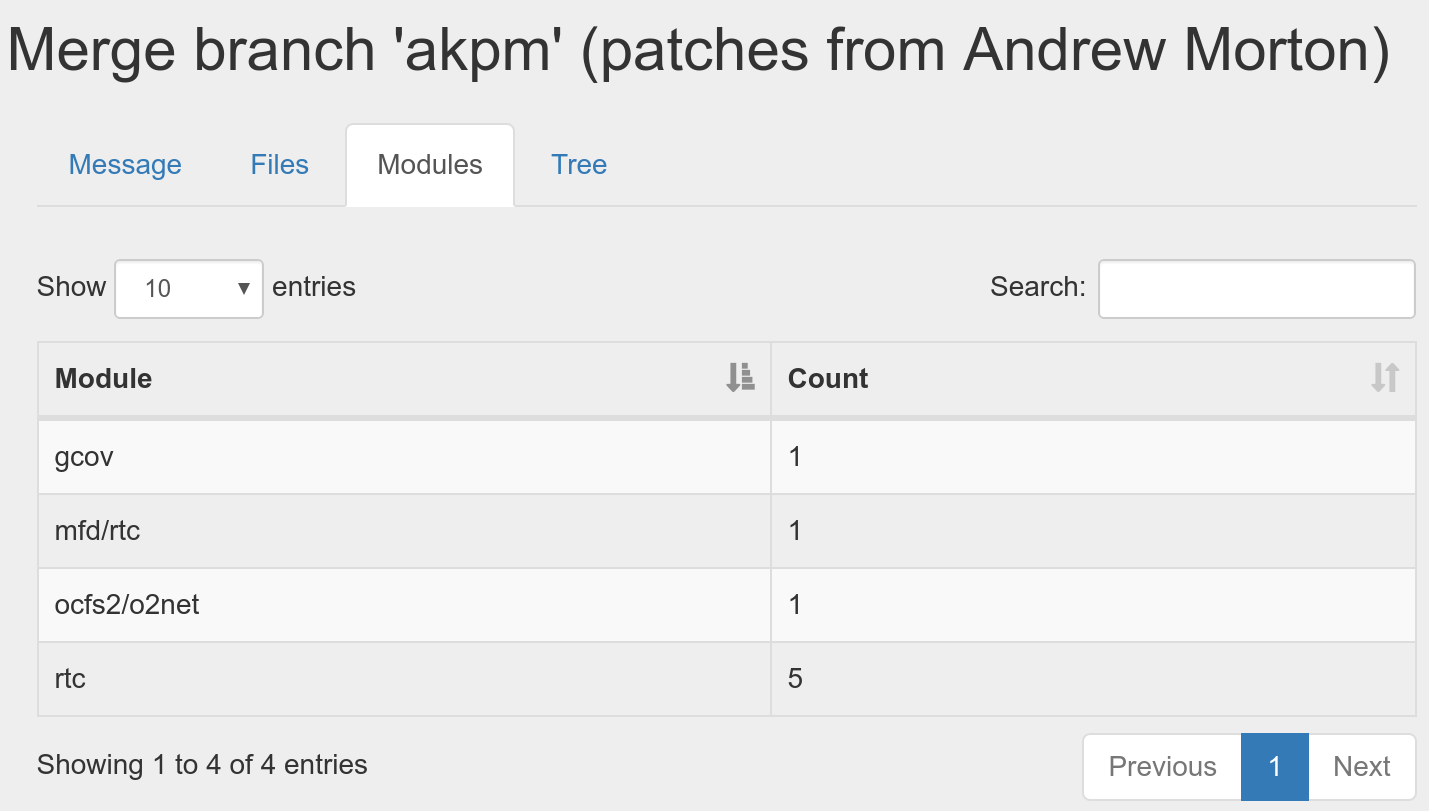
\includegraphics[width=0.47\textwidth]{figures/modules_view_2.png}
        \caption{Panel showing the modules changed by all the commits in this merge.}
        \label{fig:modules}
\end{figure}

The modules tab (Figure~\ref{fig:modules}) shows the modules that are contained
within the commit. Modules are not natively recognized by Git, and are not going to
be present in all repositories. In the Linux repository, authors put the module they
are working on in the one-line summary of the log-message; for example: the log
\emph{gcov: add support for FCC 4.9} has updated the \emph{gcov} module (the
coverage testing tool of the kernel). We heuristically extract the module by taking
all text in the log summary of commits until the first colon.  Modules are logical
partitions of the information in the kernel. Depending on where the author was
working, modules can be general, such as ``bluetooth'' and ``wireless'', or can be
quite specific for individual hardware, such as ``ath9k\_hw'' and ``wl1251''. In a
few cases, the author of a commit does not correctly follow this format and the
heuristic approach fails. As with the Files panel, non-merge commits show their
corresponding information, but for merge commits we aggregate all the modules
changed in all the commits that are part of that merge.  The output of this view is
shown in Figure~\ref{fig:modules}.

Finally, we have the Tree view tab. The tree view is designed for providing easy
navigation of the commits within the merge-tree that is rooted in the current merge.
It also provides a clear topological view of the merge and the submerges it
includes. We have experimented with various tree designs to find a design that
allows for easy navigation and visualization of both large and small trees. We
discuss this panel in the next subsection.

\subsection{Merge-Tree Views} \label{treeview_section}

The merge-tree view is what makes \tool unique to other tools that inspect the DAG
of a Git repository. With it, a user can inspect how commits are merged on their way
to the master branch. We have experimented with various types of trees:

\begin{enumerate}
        \item List trees are a text-based representation of the merge-tree, and are easy to search and navigate.
        \item Reingold-Tilford trees provide a clear visual representation of the tree structure of the merge-tree.
        \item Bubble trees organize the data hierarchically by having the parent node contain the child nodes similarly to tree maps, but
                clearly showing the parent-child relationships between commits and merges.
\end{enumerate}


\subsubsection{List Tree}

The list tree viewer (Figure~\ref{fig:list_tree}) is in the form of nested lists,
and is designed to more closely model the tree view found in file browsers. This
tree only contains the commits and merges that are within the subtrees of the
current merge. A commit will never have any items in this tree as it is a leaf. To
accompany the tree, we include breadcrumbs at the top of the page to enable a user
to navigate both from the root to the leaves and from a leaf to the root. The last
item in the breadcrumb list is the current commit, the previous item is the parent
of the current commit, and the first item is the root merge into the kernel.

\begin{figure}
        \centering
        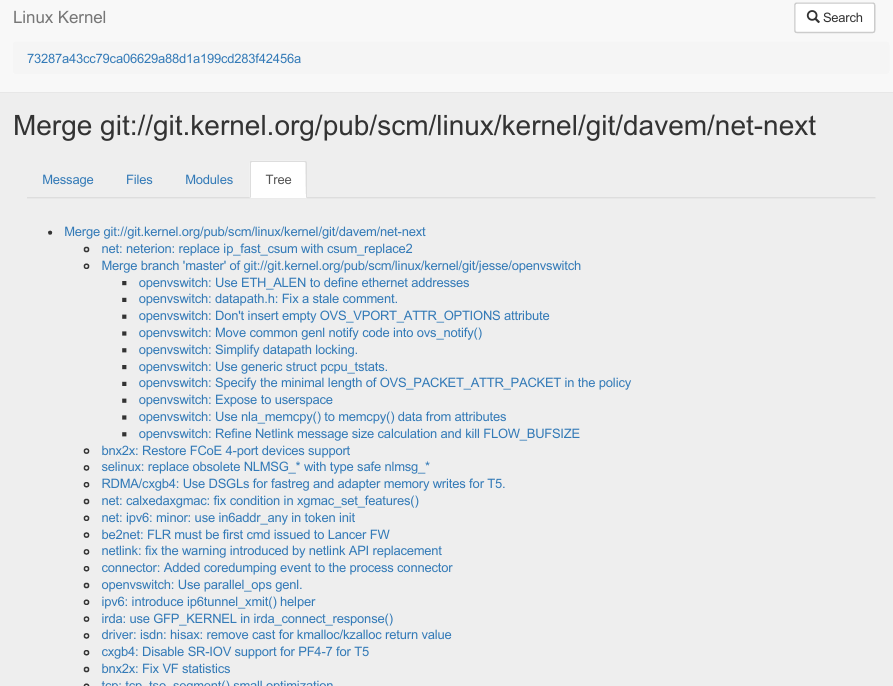
\includegraphics[width=0.47\textwidth]{figures/list_tree.png}
        \caption{List tree view of merge 3f17ea6}
        \label{fig:list_tree}
\end{figure}

\subsubsection{Reingold-Tilford Tree}

The Reingold-Tilford tree\cite{Reingold1981} (Figures \ref{fig:reingold_tree} and
\ref{fig:reingold_tree_zoom}) allows the visualization and navigation of the entire merge-tree in
an intuitive representation of the tree.  This illustrates a clear notion of root
and leaves, and how to navigate in either direction. Some merge trees are very
large, containing thousands of commits and merged. While the tree is capable of
producing a visualization, it becomes far more difficult to understand. For example,
the merge, 3f17ea6 performed by Linus Torvalds June 8 2014, contains 7217 commits
and merges. \footnote{This commit can be inspected at
  \url{http://li.turingmachine/org/commits/3f17ea6dea8ba5668873afa54628a91aaa3fb1c0}}

      \begin{figure}
        \centering
        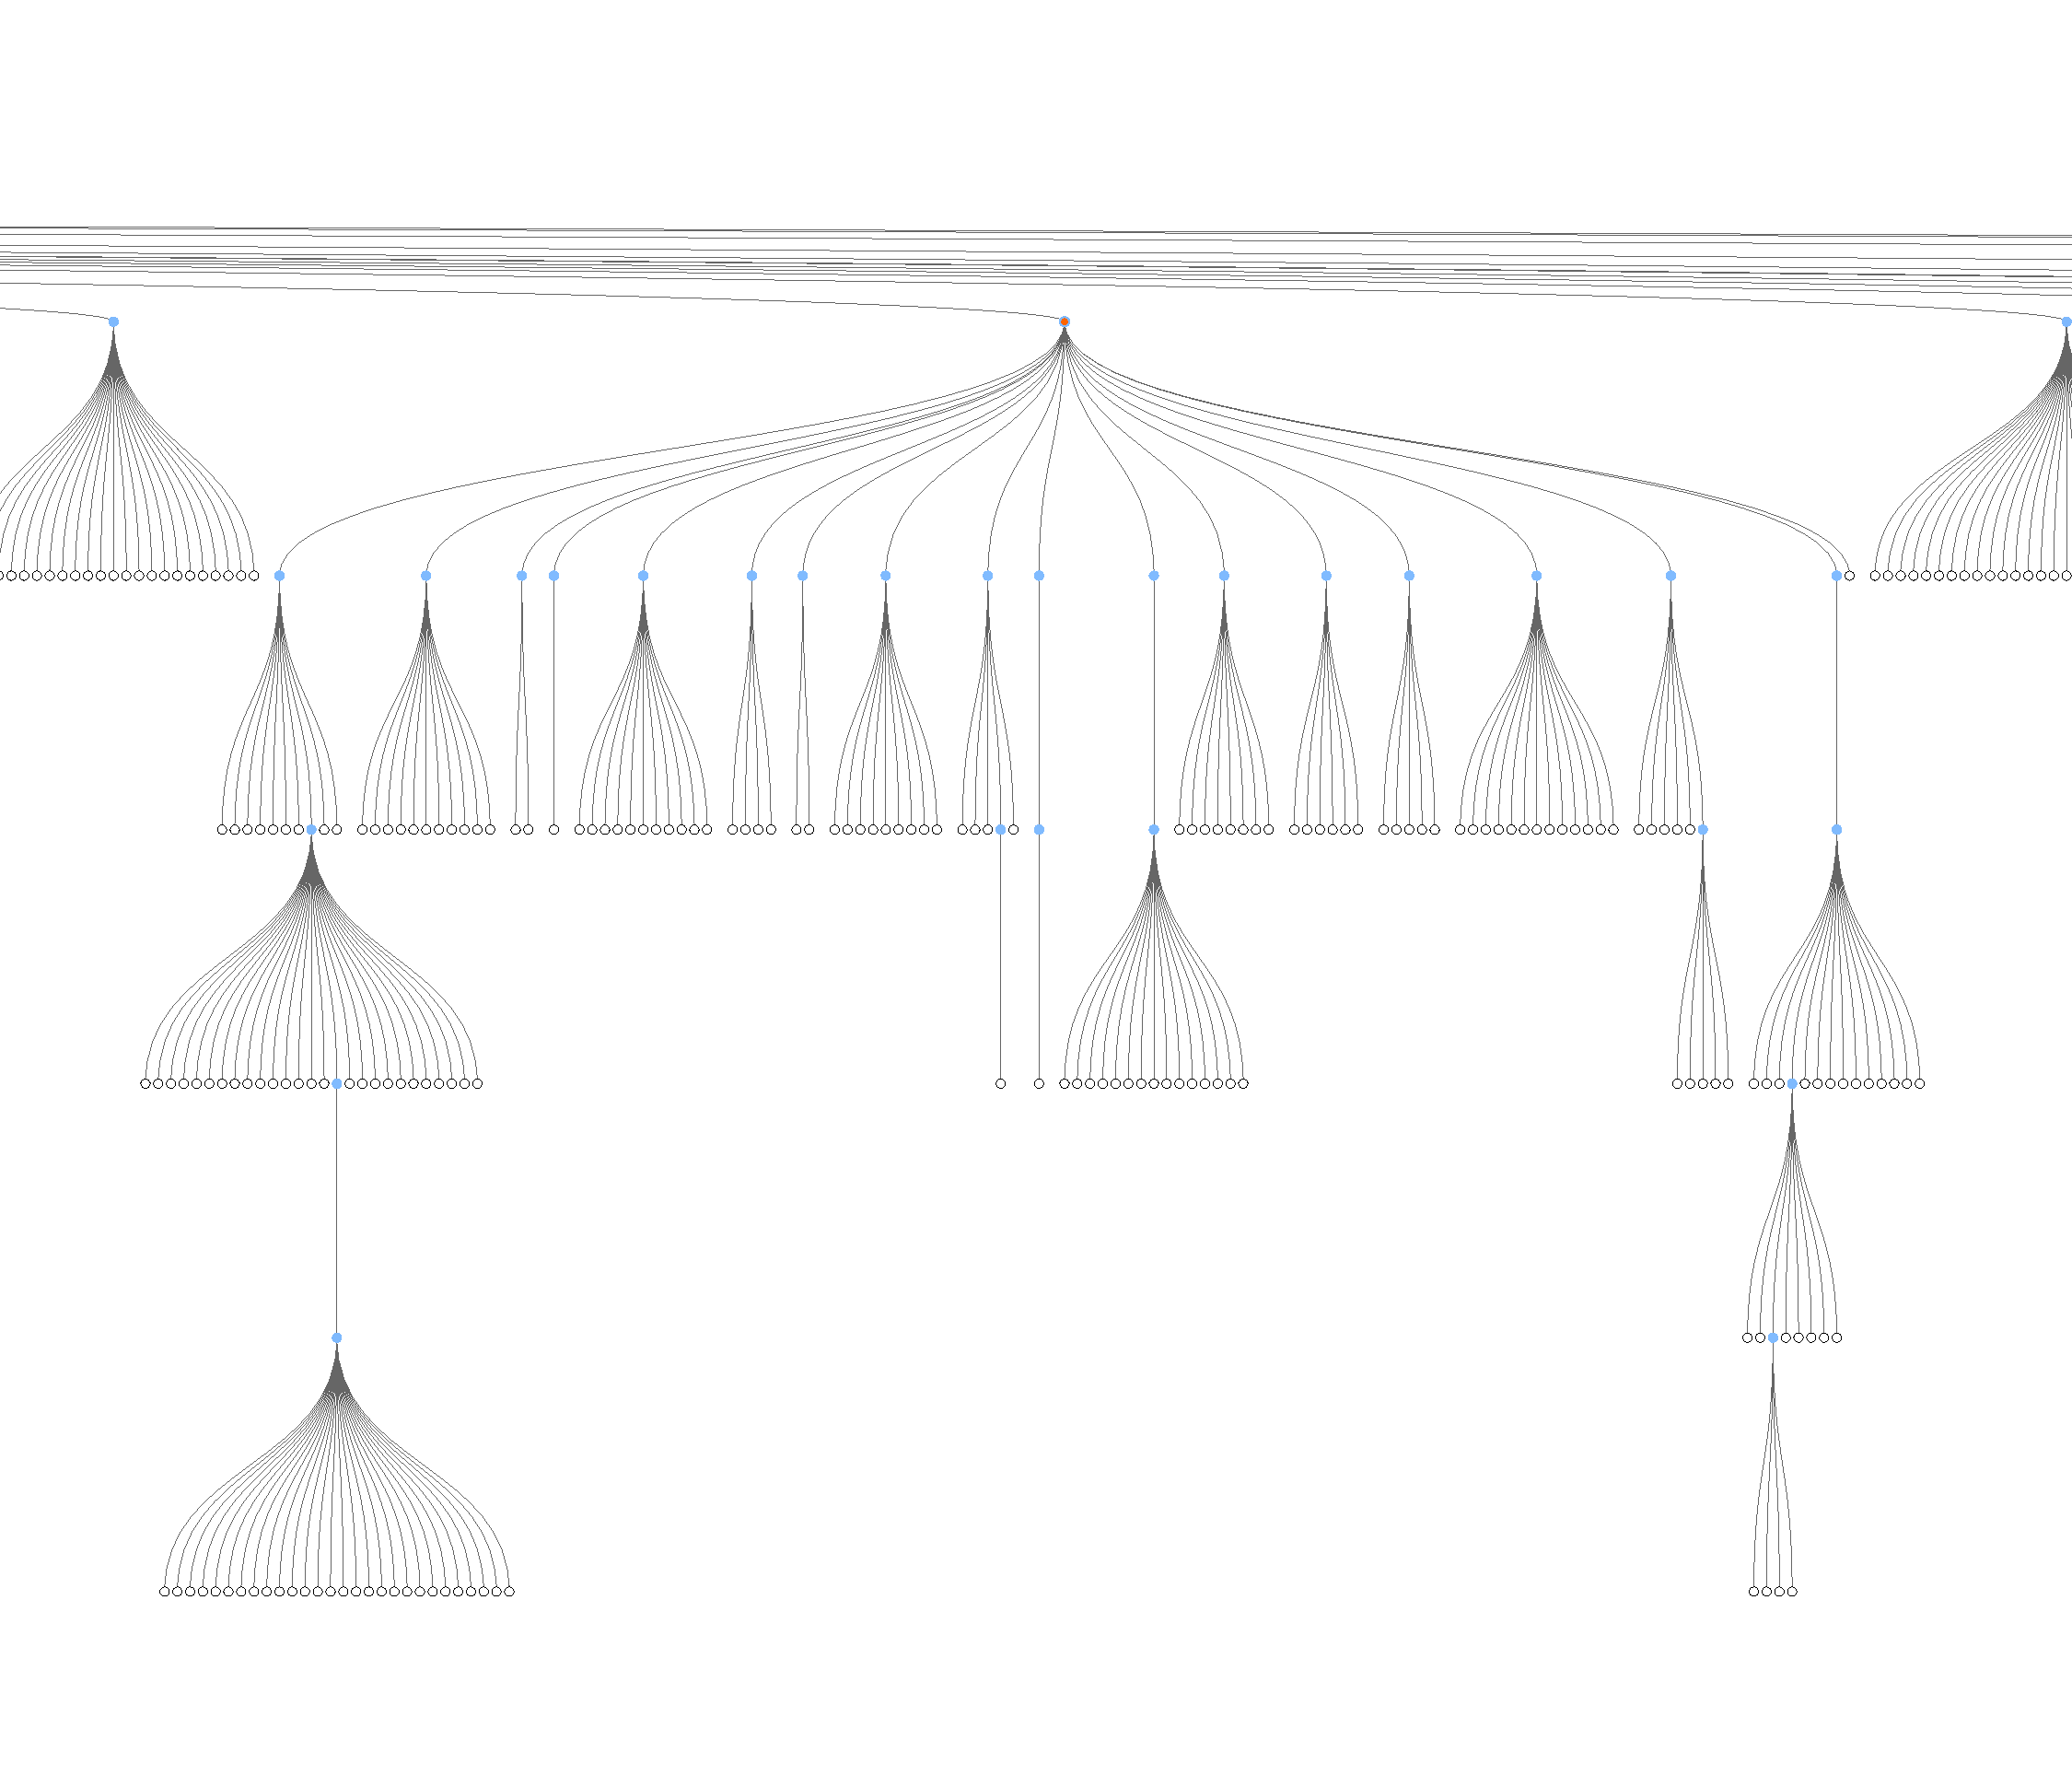
\includegraphics[width=0.47\textwidth]{figures/4dc4_tree.pdf}
        \caption{Merge 4dc4226 is a subtree of 3f17ea6, for the power-management
          module of the kernel}
        \label{fig:reingold_tree}
      \end{figure}

      \begin{figure*}
        \centering
        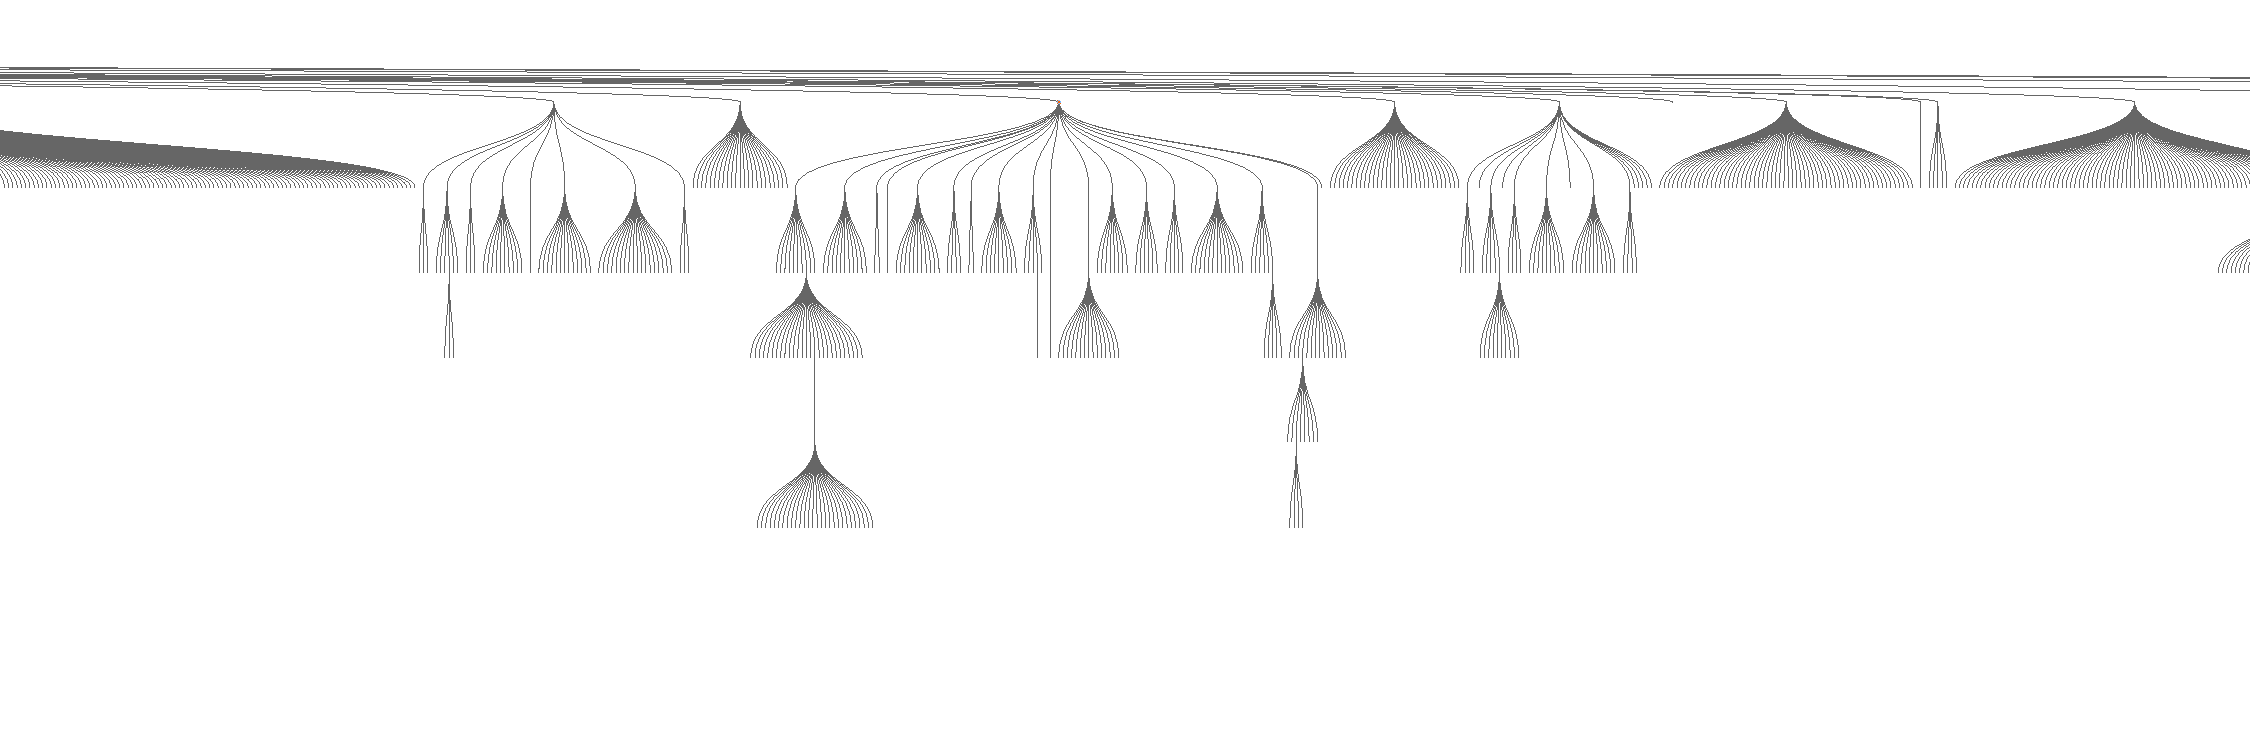
\includegraphics[width=0.98\textwidth]{figures/4dc4_zoom_tree.pdf}
        \caption{Zoomed out view of the Reingold-Tilford tree for merge 4dc4226}
        \label{fig:reingold_tree_zoom}
      \end{figure*}

      The user is initially greeted with their current node centered on the screen.
      They are able to zoom the tree by scrolling the mouse, and clicking and
      dragging to pan the tree. They can see more details about a node by clicking
      on it, which will provide them a link to the specific page for that commit.

\subsubsection{Bubble Tree}

Bubble trees are useful for providing a clear visualization of wide, hierarchical
data\cite{Boardman2000}. The tree structure is represented by the nesting of nodes;
the largest circle is the root, containing all the other nodes. The smallest circles
do not contain any nodes and therefore represent the leaf nodes.

Our implementation of the bubble tree (Figure~\ref{fig:bubble_tree}) provides the
user with a clear picture of where a commit is located in the merge tree. We
highlight the selected commit or merge in red. Non-selected merges are in a shade of
blue determined by the depth of a node in the tree. The root is the lightest shade
of blue, while the contained merges are progressively darker; the commits are white.

\begin{figure}
        \centering
        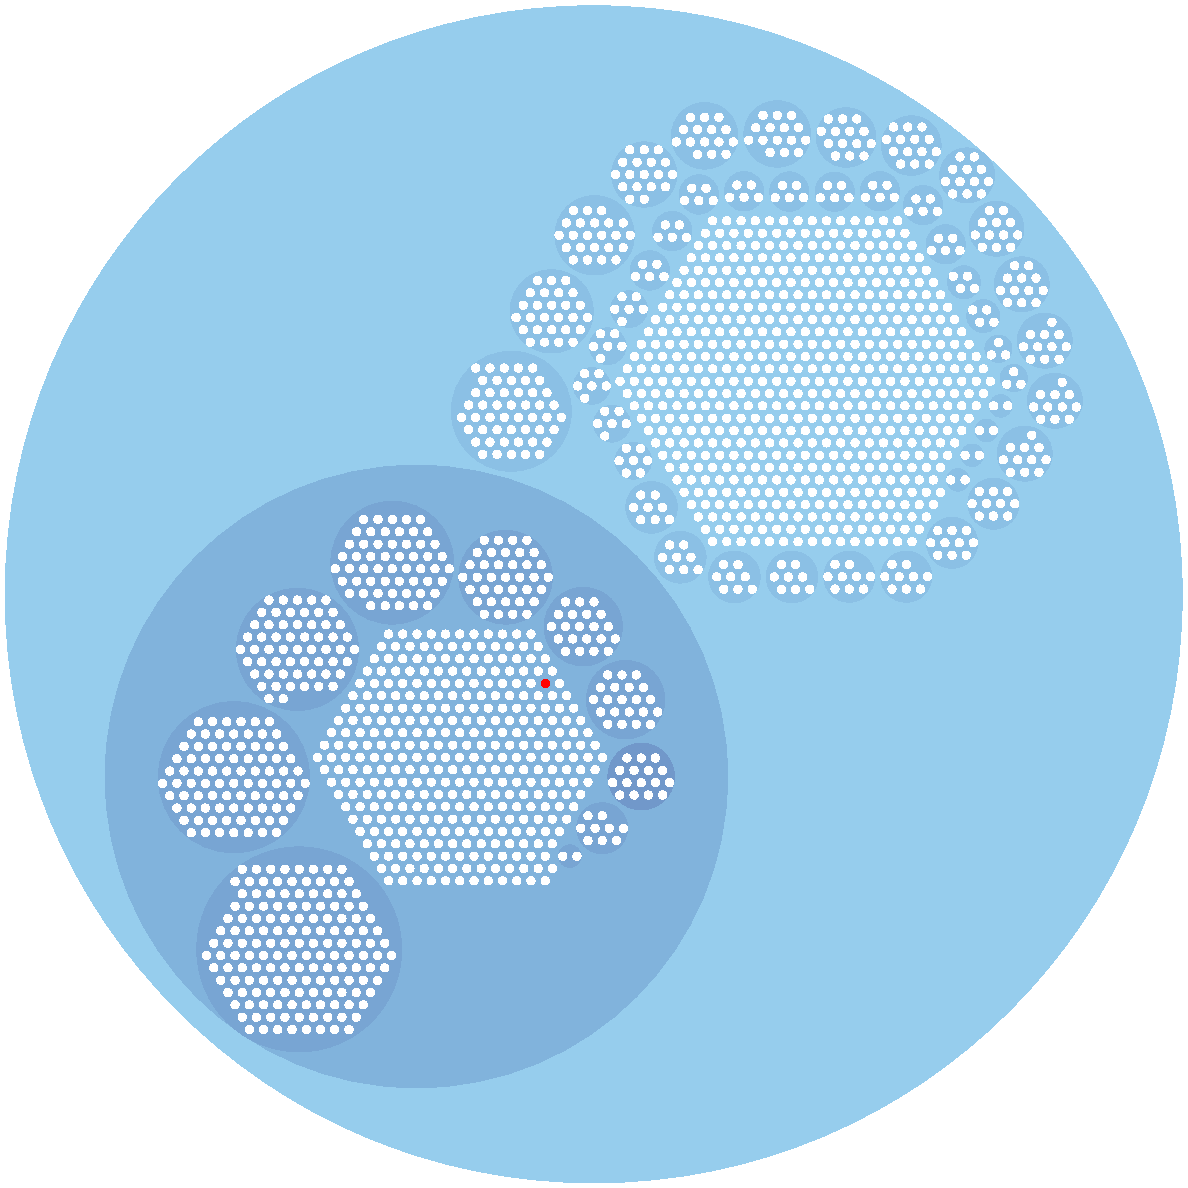
\includegraphics[width=0.47\textwidth]{figures/bubble_tree.pdf}
        \caption{Bubble Tree of merge 3f17ea6, merge 4dc4226 is the currently
          selected merge and is highlighted in orange.}
        \label{fig:bubble_tree}
\end{figure}

The bubble tree doesn't have an implicit way of providing additional information,
placing any text near the nodes makes the tree impossible to read, so we include a
separate pane in the web page. When a user hovers over a node, the pane shows
additional information about the author and the commit message and a link to the
detailed page for that commit or merge. If the user clicks on a node, the tree will
zoom to that node and the information in the info pane will persist, enabling the
user to click the link. This tree provides an easy mechanism for users to navigate
from the root to the leaves and vice versa.

\section{Implementation Details}

\evantodo{See if we can move API section to be part of another section}

The front-end uses asynchronous requests to gather the information for the trees and
tables. This enables third-parties to implement new front-ends, trying other
designs, though this interface may change in the future. The tree, file, and module
information is accessible through
http://li.turingmachine.org/data/tree/JSON/\verb|<cid>|,
http://li.turingmachine.org/data/files/JSON/\verb|<cid>|,
http://li.turingmachine.org/data/modules/JSON/\verb|<cid>|, respectively.

The response for the tree is a single object. This object is the root node of the
tree, and may contain an object of children sub-tree objects in the \verb|children|
field, which are in the same format as the root object. The children object uses the
commit ID as the key.

The tree node objects have the following fields:

\begin{tabular}{ccl}
        Field name      & Data type & Description\\\hline
        \verb|cid|      & string    & Commit ID\\
        \verb|name|     & string    & One-line log summary\\
        \verb|mlinus|   & string    & Root merge commit ID\\
        \verb|author|   & string    & Author name and email\\
        \verb|mnext|    & string    & Parent merge commit ID\\
        \verb|children| & object    & Object of tree objects\\
\end{tabular}

The file responses contain only the files that the selected merge or commit works
with. The response is a single object in the form of a tree. This object is the root
of the tree, and represents the current merge or commit. If the current position in
the tree is an inner node, the response will contain the child nodes in the
\verb|children| field, otherwise \verb|children| will be an empty list. The format of file
response is as follows,

\begin{tabular}{lll}
        Field name & Data type & Description\\\hline
        \verb|cid| & string & Commit ID\\
        \verb|mnext| & string & Parent merge commit ID\\
        \verb|children| & list & List of tree objects\\
        \verb|files| & list of tuples&
        \footnotesize{
                \begin{tabular}{lc}
                        \verb|Filename| & string\\
                        \verb|Lines added| & uint\\
                        \verb|Lines removed| & uint\\
                \end{tabular}}\\
\end{tabular}

\section{Discussion}

From a developers point of view, the are two major disadvantages of the DAG model of
Git: a) its edges point backwards, i.e. commits point to their ancestor, not to the
commit that succeeds them on the path to being integrated; and b) the DAG contains
many more edges that are necessary to understand how integration occurred. We
addressed these two issues with the creation of the merge-tree model from the DAG of
Linux. Effectively, the merge-tree recovers the details of how each branch---and the commits they contain---was merged
into the master branch.

In our experience, no other Git repository reaches the level of DAG complexity that
Linux has. In most Git repositories, most merges are not nested---most merges merge
directly into the master repository, and these merges only merge a few commits. Even
in these simplified cases, the merge-tree can provide a valuable summary of how
commits are integrated into the master branch, specifically since the time of
integration may be very different from the time the commits were authored.

\evan{Check accuracy of this paragraph}

The biggest challenge is computing the merge-tree of any given repository. It
is likely that our heuristic for computing the merge-tree will not work with other
repositories. The heuristic requires that there are no fast-forward merges into the
master branch of the repository (a majority of repositories), and that there are no
foxtrot merges (a practice that is starting to be considered desirable by git users\footnote{See
  \url{http://devblog.nestoria.com/post/98892582763/maintaining-a-consistent-linear-history-for-git} and
  \url{https://developer.atlassian.com/blog/2016/04/stop-foxtrots-now/}}).
We are able to use our heuristic with the Linux kernel because of
the strict integration model imposed by Linus. To validate the results of the
heuristic, we use the continuous mining technique described in \cite{German2015}.
Continuous mining of the repository requires foresight and planning.

Because \tool leverages the merge-tree model of the kernel, it provides mechanisms
and visualizations that other tools are unable to produce. It gives us the ability to
see how commits are being merged into the master branch, allowing us to better understand
how code is integrated into the kernel.

\begin{figure}
        \centering
        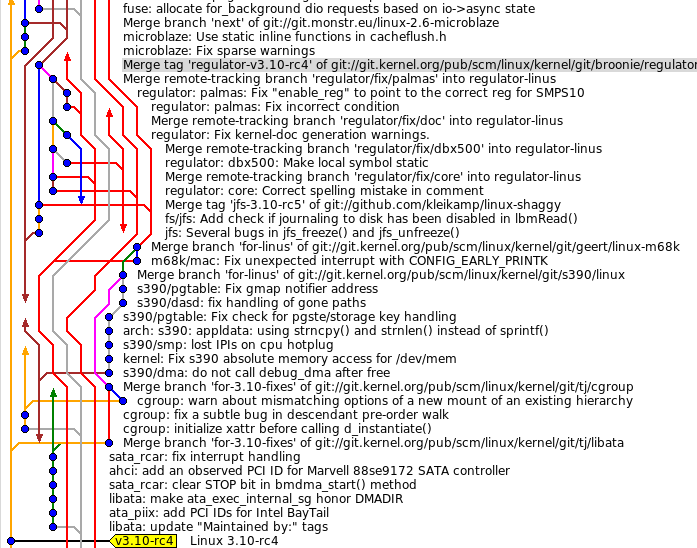
\includegraphics[width=0.47\textwidth]{figures/042dd_DAG.png}
        \caption{Merge Dag View}
        \label{fig:dag_view}
\end{figure}

\begin{figure}
        \centering
        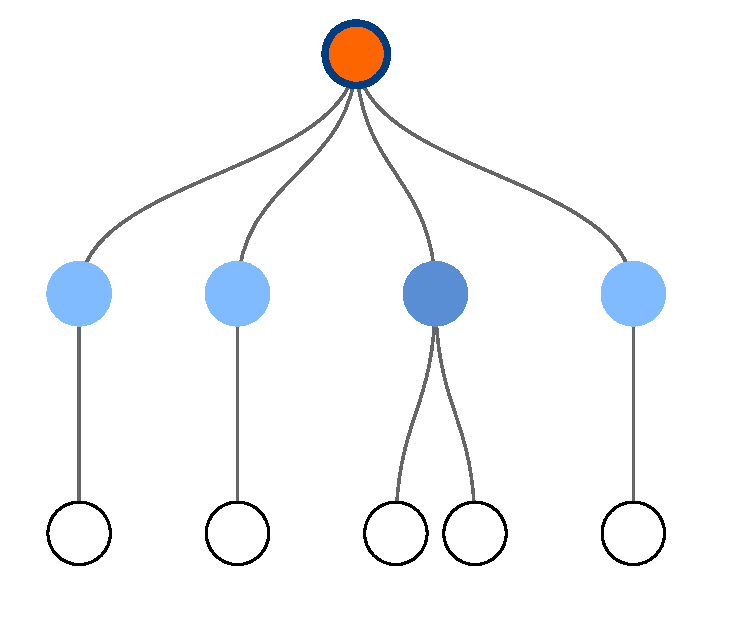
\includegraphics[width=0.47\textwidth]{figures/042dd_tree.pdf}
        \caption{Merge tree topology for the same merge as in
                Figure~\ref{fig:dag_view}.}
        \label{fig:tree_view}
\end{figure}

Our goal was to build a tool to enable maintainers to effectively navigate and
browse the changes performed to the kernel over the period of a release. Achieving
this goal includes removing information that does not pertain to the area of the
kernel that the user is interested in. In Figures~\ref{fig:dag_view} and
\ref{fig:tree_view} we can visually compare the results returned from Gitk
and our tool for the top-level merge ``042dd60ca6dec9a02cefa8edd67de386e35755d6''
from kernel version 3.10. Note that Gitk has no way to show or recognize that this
is a merge into the master branch.

The log information to this merge-commit in both of these figures is identical, but
the presentation drastically changes our ability to comprehend what we are seeing.
The primary difference is the removal of irrelevant information. In Gitk
(Figure~\ref{fig:dag_view}), the visualization results include commits and merges
from other components of the kernel, while our tool (Figure~\ref{fig:tree_view})
only includes the results that are specific to the component of the kernel that we
are interested in.

Even though this merge is relatively small, containing only four sub-merges, three of which
only contain a single commit, and the last containing two commits, it is already hard to visualize in Gitk.
With \tool we are able to immediately see what section of the kernel these commits and merges pertain to. The DAG view of this provides almost no explanation,
furthermore, users must work to determine where this merge ends and the next one
begins.

\tool further enhances our understanding by summarizing the files
and modules that were edited in the entire branch being merged. We are able to determine that three
files, ``palamas-regulator.c'' had two lines added and two lines removed,
``dbx500-prcmu.c'' had 12 lines added and 12 lines removed, and ``core.c'' had 5
lines added and 2 lines removed. Finally, we are able to determine that only the
``regulator'' module was modified in this merge and was modified by 5 commits.

\section{Future Work}

There are still many areas that can be improved before the full potential of our
model can be realized. Here, we outline various areas of the tool that still need
more attention.

\subsection{Files}

There currently is no functionality surrounding searching by filename. Users falling
under use-case 2 may know what file they are editing and try to determine how it may
work with the other commits and merges in the module. It is possible that a third
use-case may arise, where the user wants to determine all commits that effect a
given file. In both cases, bottom-to-top approach is applied.

There is limited functionality to the presentation of the file information. At a
minimum, the patches for the commits can be displayed. From there, the patches can
be used to piece together parts of the file to generate a single patch at a given
merge rather than displaying each patch individually. The patches can also be used
for determining what kinds of changes were made, if the lines are being added,
removed, or being replaced.

\subsection{Authorship}

Our model can aggregate more information than what we have implemented. The
authorship information is important for licensing purposes, and we can show all
authors contributing to commits in a  merge and how many commits they contributed to
the merge. We could go further, providing information about what files they edited,
how many lines they added and removed, and more.

\subsection{Evaluation}

At this time, we have no evidence that our tool is able to improve the work-flow of
maintainers. We believe that the tool is able to improve the work-flow and
performance of maintainers because it provides cleaner mechanisms of visualizing and
presenting the commit information. It is able to provide more relevant information,
while removing information that is irrelevant to a given module or set of merges.

We can either perform user-testing to show how a users workflow changes, or we could
have maintainers evaluate and critique the tool and use their feedback to determine
if the tool meets our goals.

\section{Related Work}

Version control systems monitor the development lifetime of software projects. This
makes the version control system vital in providing information about how a software
project is being developed. To our knowledge, we know of no Git repository
visualization tool that builds a tree that maps the path a commit follows to the
master branch from the DAG provided by Git. This may be because more information is
required to generate the merge-tree model than what is stored by Git. However, there
has been a lot of work in providing visualizations of various repositories.

Many tools work to address the issues in communication between developers in
inter-team collaboration work. Codebook \cite{Begel2010} uses a data mining
technique  to determine the developer of a piece of code, the program manager who
wrote the specification for the code, and the program managers and developers on the
team who were working together. Hipikat\cite{Cubranic2005} is another tool with a
focus on communication. Where Codebook focuses on developers working on a project,
Hipikat is focused on enabling easier integration of new developers to a project by
providing them with easily-searchable artifacts of the changes made. Codebook is
useful for pairing a contributor with the original developer; however, the developer
may not have worked with the piece of code in years. A Hipikat program may provide
more information to the maintainer as it records the artifacts of why certain
design decisions were made when they were made using other tools like Bugzilla and
CVS. Neither tool is sufficient in meeting our goals to provide a summary of the
topology of the kernel repository through a visual tree.

Most visualizers provide a visual presentation of a certain aspect of a repository.
Fractal Figures \cite{Ambros2005} uses a unit square to represent a portion of a
project, then partitions the square based on the proportion of an author's
contributions to that portion of the project. EPOSee\cite{Burch2005} and Evolution
Radar\cite{Ambros2009} perform further analysis, determine which files are made
together, and what changes are made over a sequence of commits, though the goals
behind these projects is different.

Codebook, Hipikat, Fractal Figures, EPOSee, and Evolution Radar all work with data
from CVS repositories. Our goal is to provide information about Git repositories,
specifically the Linux master repository. Fewer tools are available for generating
visualizations and summaries of Git repositories, potentially due to the DAG model
used by Git.

Gource is a tool for providing an interactive timelapse of the state of a
repository\cite{Caudwell2010}. In the timelapse, it shows who contributes and what
type of contribution a developer is making. These contribution types are one of,
adding a file, removing a file, and changing a file. While the timelapse is
interesting to watch, it does not provide any additional explanation of the changes
actually being made, only the frequency that they are being made and who is making
them.

The current industry standard tool for Git repository visualization is Gitk. The
Gitk interface is built around the central DAG viewer. The DAG view displays the
commits on their respective branches, the author of the commit or merge, and the
date the commit or merge was authored. A user can select a single merge or commit
to view additional information. For both merges and commits, Gitk will present the
user with the Git log. If the user selected a commit, Gitk will also present the
user with the patch information and the names of the files edited. Gitk is unable to
provide the patches and filenames information in merges, as it is unable to
aggregate commit information in merges.

Our tool is primarily aimed at presenting the hierarchical structure of the Linux
git repository. We use tables for presenting the summarized information of the
commits and merges, but this information could also be presented in a graphical
form. Various graphical forms for displaying file and authorship data exist, the
principal forms being matrix views, city scapes, bar and pie charts, and networks
\cite{Eick2002}. Any of these data visualization metaphors are applicable to our
system.

\section{Conclusion}

Our tool, \tool, shows promising results in working toward our goals, building a tool that
can more easily navigate the repository, and provide clearer explanations of the
changes made. The filtering by searches and the various tree visualizations enable
users to easily navigate through the kernel, finding the commits and merges that
pertain to what they are interested in. The tree visualizations are able to both
serve as a navigation piece, providing simpler navigation through the kernel, but
also demonstrate which commits contribute to which merges, providing further
explanation over the DAG. The tree model further improves the explanation by enabling
the tool to aggregate metadata at the merges instead of requiring a user to manually
aggregate the information. Our tool currently aggregates file information and the
modules edited, but can be extended to include authorship information and aggregated
patch information.

\evan{Check the validity of this paragraph}
We use a heuristic method to generate the tree from the repository. The heuristic
requires that the repository does not have fast-forward merges into the master
branch or foxtrot merges, which obfuscate the master branch. In either case, the
heuristic will break and result in a tree that does not accurately represent the
repository.

These may pose as significant drawbacks to smaller projects; however, with a proper
merge discipline, the heuristic is able to correctly convert the DAG into a
merge-tree. The importance of clear visualizations in large projects outweighs
the costs of enforcing a clean merge discipline. The tree-based model appears to
have the ability to provide a clean visualization and more detailed explanations of
the changes in the Linux kernel.

% \nocite{*}

\bibliographystyle{IEEEtran}
\bibliography{citations}

\end{document}

%%% Local Variables:
%%% mode: latex
%%% TeX-master: t
%%% End:
